\section{Analiza wymagań}
System skierowany jest do firm zajmujących się wytwarzaniem produktów IT. Skierowany jest do wszystkich zatrudnionych w firmie, z głównym wskazaniem na:
\begin{itemize*}
\item menadżerów projektów,
\item pracowników technicznych (programistów, testerów)
\item analityków.
\end{itemize*}

System ma za zadanie wspomaganie zarządzania projektami oraz zasobami niezbędnymi do ich wytwarzania. Ma umożliwiać stałe monitorowanie postępów projektu. Ma zapeniać możliwość szybkiej reakcji na zmiany (odejście/choroba pracownika, wcześniejsze/późniejsze zakończenie projektu).

\subsection{Wymagania funkcjonalne}
Głównym zadaniem systemu jest wsparcie zarządzania projektami pod kątem:

\begin{tabularx}{\textwidth}{|c|X|X|c|}
\hline 
Lp. & Nazwa & Opis & Priorytet \\ 
\hline 
\multicolumn{4}{|c|}{\textbf{Zarządzanie personelem}} \\
\hline 
F001 & Uwierzytelnianie & Aplikacja umożliwia uwierzytelnianie osób korzystających z systemu  & Wysoki \\ 
\hline 
F002 & Zarządzanie uprawnieniami & System umożliwia tworzenie kont z różnymi poziomami uprawnień & Wysoki \\ 
\hline 
F003 & Walidacja poziomu uprawnień & System dostosowuje widoczne dla użytkownika opcje w zależności od poziomu uprawnień użytkownika  & Wysoki \\ 
\hline 
F004 & Zarządzanie pracownikami & System umożliwia dodawanie usuwanie i modyfikację kont pracowników. W ramach konta jednego pracownika system umożliwia wprowadzenie: \newline
- danych personalnych \newline
- kwalifikacji \newline
- historii zatrudnienia \newline 
- stawki \newline
- informacji o stanowisku
& Wysoki \\
\hline 
F005 & Zarządzanie strukturą organizacyjną firmy & Program umożliwia przeglądanie zależności stanowisk-owych pracowników firmy. System umożliwia tworzenie, usuwanie i modyfikacje elementów tak rozumianej struktury firmy. & Wysoki \\ 
\hline 
F006 & Zarządzanie czasem pracy pracowników & System umożliwia tworzenie raportów przez pracownika dotyczących przepracowanego czasu na poszczególnych zadaniach. W szczególności system umożliwia wprowadzenie informacji o stanie zaawansowania prac nad zadaniem którego dotyczy raport. & Wysoki \\ 
\hline 
\multicolumn{4}{|c|}{\textbf{Zarządzanie projektami}} \\
\hline 
F101 &  Tworzenie projektu & System umożliwia tworzenie i usuwanie projektów. System umożliwia wprowadzenie oraz modyfikację danych projektu np. status projektu. & Wysoki \\ 
\hline
F102 & Terminarz projektu & Dla każdego projektu system umożliwia tworzenie usuwanie i modyfikację terminarza projektu & Wysoki \\
\hline 
F103 & Definiowanie zadań & Dla każdego projektu system umożliwia dodanie i usunięcie zadania. System umożliwia także modyfikowanie danych zadania np. nazwa zadania, opis zadania & Wysoki \\ 
\hline 
F104 & Wymagania projektu & System umożliwia przypisanie do projektu kwalifikacji które musi posiadać zespół, aby można wykonać zaplanowaną pracę . & Wysoki \\ 
\hline 
F105 & Wyszukiwanie członków zespołów & System umożliwia wyszukanie pracowników o odpowiednich kwalifikacjach. Dla każdego znalezionego pracownika system pokazuje informacje o aktualnym obciążeniu pracownika& Wysoki \\ 
\hline 
F106 & Alokacja pracowników do projektów & System umożliwia przypisanie pracownika do projektu. & Wysoki \\ 
\hline 
F107 & Obciążenie pracowników & System udostępnia informacje o obciążeniu każdego z pracowników, czyli w nad jakimi projektami pracuje, oraz na jaki czas pracownik został 'zarezerwowany' w związku z danym projektem & Wysoki \\ 
\hline 
F108 & Zarządzanie kosztami projektów & System umożliwia: \newline
- definiowanie kosztów poszczególnych pracowników \newline
- zatwierdzanie raportów czasu pracy pracowników. & Wysoki \\
\hline
\multicolumn{4}{|c|}{\textbf{Monitorowanie statusu projektów}} \\
\hline 
F201 & Monitorowanie kosztów & System automatycznie informuje o przekroczeniu planowanych kosztów zadań lub całego projektu & Wysoki \\ 
\hline 
F202 & Zaawansowanie pracy & System automatycznie określa stan prac na podstawie danych podanych w raportach pracowników & Wysoki \\
\hline 
F203 & Podgląd zaawansowania pracy & Program pozwala na podgląd zaawansowania prac nad całym projektem oraz w rozbiciu na poszczególne zadania & Wysoki \\
\hline 
\multicolumn{4}{|c|}{\textbf{Zarządzanie systemem}} \\
\hline 
F301 & Generowanie profili & Program pozwala generować profile umiejętności kandydatów.  & Średni \\ 
\hline
F302 & Archiwizacja danych & System umożliwia archiwizacje danych związanych z projektami & Średni \\ 
\hline
\end{tabularx} 


\subsection{Wymagania niefunkcjonalne}
System ma zapewniać:
\newline
\begin{tabularx}{\textwidth}{|c|X|X|c|}
\hline 
Lp. & Nazwa & Opis & Priorytet \\ 
\hline 
\multicolumn{4}{|c|}{Bezpieczeństwo}\\
\hline
NF001 & Uwierzytelnienie użytkowników & W celach autoryzacji użytkownika jest niezbędne zastosowanie mechanizmów z wykorzystaniem prokołu zabezpieczającego połączenie (np. SSL). & Wysoki \\ 
\hline 
NF002 & Brak możliwości dostępu osób nie autoryzowanych & Podział ról (np. administrator) ma zapewniać zestaw odpowiednich uprawnień, dzięki którym użytkownik może dostać się do modułów systemu zgodnych z jego kompetencjami. & Wysoki \\ 
\hline 
NF003 & Możliwość skorzystania z aplikacji przy korzystaniu jedynie z sieci lokalnej firmy & Brak możliwości skorzstania z aplikacji, poza placówką firmy (nie dotyczy korzystania z usługi VPN). & Wysoki \\ 
\hline 
NF004 & Wymaganie od użytkownika stosowania złożonych haseł & Użytkownik w celu zachowania bezpieczeństwa swojego konta oraz danych systemu ma używać haseł złożonych z minimum 8 znaków, w których skład wchodzą duże i małe litery, oraz liczby. & Wysoki \\ 
\hline 
NF005 & Szyfrowanie danych w bazie & W razie sytuacji ataku i kradzieży danych należy zapewnić aby baza z poufnymi danymi użytkowników nie była rozszyfrowywalna przez osoby postronne. & Wysoki \\ 
\hline 
NF006 & Przechowywanie informacji (logów) dotyczących użytkowania systemu & Prowadzenie dzienników daje możliwość wglądu w opatrzony dokładnymi datami spis działań na systemie i jego środowisku (np. czas użytkowania, adresy ip). Dzięki temu w razie ataku możliwe jest odtworzenie towarzyszących zdarzeń. & Średni \\ 
\hline 
\multicolumn{4}{|c|}{Dostępność}\\
\hline 
NF107 & System ma być dostępny dla użytkowników w czasie godzin pracy zgodnych z ustalonymi normami & System powinien być dostępny w godzinach pracy, oraz poza nimi (w przypadku dodatkowych terminów, lub nienormowanego czasu pracy). System może być niedostępny 3 dni w skali roku - ze względu z zaplanowanymi pracami (utrzymanie, aktualizacja) oraz czasu reakcji na awarie, z preferencją na noce i dni wolne od pracy. & Wysoki \\ 
\hline 
NF108 & System powinien zapewniać szybką reakcję na działania użytkownika & System powinien reafować w ciągu 5 sekund na działania użytkownika (poza obciążającymi zadaniami jak np. generacja raportów). & Średni \\ 
\hline 
\multicolumn{4}{|c|}{Reakcja na awarie}\\
\hline 
NF209 & Tworzenie wersji zapasowych & System powinien zapewniać cotygodniowe, automatyczne tworzenie bacupów, oraz możliwość przywrócenia wersji zapasowej  & Wysoki \\ 
\hline 
NF210 & Krytyczne sytuacje awaryjne powinny być automatycznie przechwytywane & Wszelkie błędy działania systemu powinny być automatycznie wykrywane i przekazywane do administratora systemu & Wysoki \\  
\hline 
\multicolumn{4}{|c|}{Skalowalność}\\
\hline 
NF311 & Możliwość obsłużenia wzrastającej ilości użytkowników i projektów & W ramach rozwoju formy system powinien być przygotowany na posiadanie zwiększonej ilości danych o pracownikach oraz nowych projektach & Wysoki \\ 
\hline 
NF312 & Możliwość obsłużenia dużej ilości zapytań & Przy rozwoju firmy ilość zapytań od użytkowników będzie wzrastać - responsywność systemu powinna zostać zachowana w granicach założonych limitów czasowych & Średni \\ 
\hline 
NF313 & Możliwość rozwoju systemu & System ma dawać możliwość dołączania nowych funkcjonalnych modułów & Wysoki \\ 
\hline
\multicolumn{4}{|c|}{Ograniczenia systemu}\\
\hline
NF414 & Udostępnienie usługi dla ilości użytkowników i projektów zgodnie z dostarczonymi zasobami & Zgodnie z ustaloną wielkością zasobów system powinien obsłużyć odpowiadającą ilość profili użytkowników, oraz projektów & Wysoki \\ 
\hline
\multicolumn{4}{|c|}{Użytkowanie}\\
\hline
NF515 & Dostarczenie intuicyjnego interfejsu użytkownika & System powinien być przeżysty i intuicyjny, nawet dla nowych użytkowników & Średni \\ 
\hline
NF516 & Łatwe poznanie dodatkowych funkcjonalności & Poznanie wszelkich bardziej skomplikowanych funkcjonalności, oraz przedstawienie systemu dla mnie obeznanych z podobnymi technologiami pracowników, powinno być możliwe dzięki około godzinnego kursu & Niski \\ 
\hline
NF516 & Dostęp ze standardowej przeglądarki & System powinien być dostępny i prawidłowo działać przy użyciu jednej z trzech standardowych przeglądarek (Chrome, Firefox, Opera) & Średni \\ 
\hline
\end{tabularx}


\section{Aktorzy systemu}
Aplikacja będzie używana przez różne osoby w firmie. W ramach aplikacji zdefiniowane są następujące role, jakie pełnione są przez użytkowników:
\begin{itemize*}
\item System
\item Administrator
\item Pracownik
\item Kierownik projektu
\item HR
\end{itemize*}
W ramach każdej roli zdefiniowany jest inny zakres możliwości i funkcji dostępnych w systemie.

\begin{figure}[h]
    \centering
    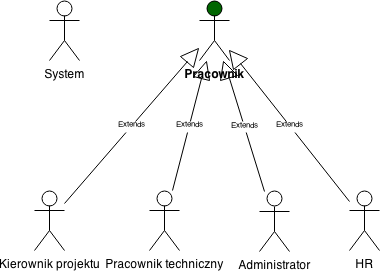
\includegraphics{diagramy/usecases/actors.png}
    \caption{Aktorzy systemu}
    \label{fig:actors}
\end{figure}
